\newpage
\section{Dual Matroids}
The concept of \textit{duality} is an interesting feature of matroid theory. It helps to extend some of the constructions in our prototypical examples in representable and graphic matroids, such as the notion of orthogonality in vector spaces and the concept of a planar dual of a plane graph, to general matroids. In this section, we will introduce the definitions and  properties of dual matroids.

%Before starting with the formal definitions, porperties and theorems is important that we state the most important concept of this chapter, that is, similar to the chapter name, the concept of a \textit{dual}, or more precisely, the \textit{dual of a matroid}.\

% I DONT THING THE ABOVE PARAGRAPH ADDS ANY CONTENT

If we have a matroid $M$, with sets $(E,\mathcal{B})$, or in other words $M$ is a matroid on $E$ with $\mathcal{B}$ as its collection of bases. Then its dual will refer to a new matroid, which we denote by $M^*$. This new matroid has the property that it is ``related'' to the original matroid, so it has the same ground set $E$ of the original matroid $M$, but a different basis set. This new basis collection will be called $B^*$. We will then define $M^*$ by the pair of sets $(E,\mathcal{B}^*)$, where $\mathcal{B}^*$ contains the complements of all bases in $\mathcal{B}$. This can be seen more clearly in the following digram:
\begin{figure}[H]
    \centering
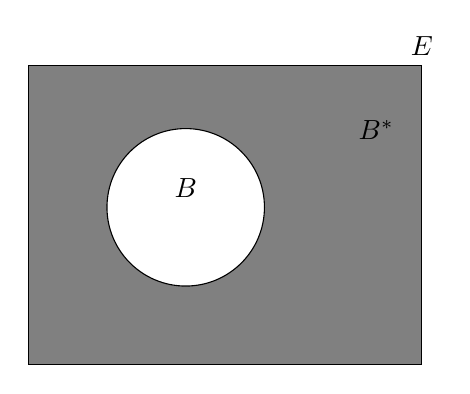
\begin{tikzpicture}
        \filldraw[fill=gray] (-2,-2) rectangle (3,1.8) node [text=black,above] {$E$} node at (19:3) [text= black, left = 2pt] {$B^*$};
        \scope % B
        \clip (0,0) circle (1);
        \fill[white] (0,0) circle (1.5);
        \endscope
        \draw (0,0) circle (1) node [text=black,above] {$B$};
\end{tikzpicture}
    \caption{Venn diagram showing a basis $B \in \mathcal B(M)$ of $M$, and a basis $B^* \in \mathcal B(M^*)$ of it's dual}%
\label{graphic}%
\end{figure}

We will consider the matroid depicted in previous sections (figure (\ref{fig:1234-matroid-circuits})). We also consider it's dual (figure (\ref{DoubleDiagramDual})). To the \textbf{left} we have the depiction corresponding to the \textbf{original matroid}, and to the \textbf{right} we have the one corresponding to its \textbf{dual matroid}. 
We notice the ground set is composed of 4 components $E=\{1,2,3,4\}$, and the original matroid has bases $12$ and $23$ (highlighed in red). Its dual has bases $34$ and $14$ respectively (also highlighted in red). This is because the complement of the elements $12$ is $34$, and the complement of $23$ is $14$.

\begin{figure}[H]
\begin{tikzpicture}[H]
\centering
\matrix (a) [matrix of math nodes, column sep=0.3cm, row sep=0.35cm,]{
 & & &\textcolor{cyan}{
1234} & & & &\\
 \textcolor{cyan}{
123}& &\textcolor{cyan}{
124} & &\textcolor{cyan}{
134} &  & \textcolor{cyan}{
234}  \\
\textcolor{red}{12} & \textcolor{blue}{13} & \textcolor{cyan}{14} & & \textcolor{red}{23} & \textcolor{cyan}{
24} & \textcolor{cyan}{
34} \\
\textcolor{orange}{1}& &\textcolor{orange}{2} & & \textcolor{orange}{3}& & \textcolor{blue}{4} \\
& & & \textcolor{orange}{\emptyset} &  & & \\
&&&&&& \\};

\foreach \i/\j in {1-4/2-1, 1-4/2-3, 1-4/2-5, 1-4/2-7, 2-1/3-1, 2-1/3-2, 2-1/3-5, 2-3/3-1, 2-3/3-3, 2-3/3-6, 2-5/3-2, 2-5/3-3, 2-5/3-7, 2-7/3-5, 2-7/3-6, 2-7/3-7, 3-1/4-1, 3-1/4-3, 3-2/4-1, 3-2/4-5, 3-3/4-1, 3-3/4-7, 3-5/4-3, 3-5/4-5, 3-6/4-3, 3-6/4-7, 3-7/4-7, 3-7/4-5, 4-1/5-4, 4-3/5-4, 4-5/5-4, 4-7/5-4}
\draw[double, line width = 0.005mm, color = brown] (a-\i) -- (a-\j);
\end{tikzpicture}
\begin{tikzpicture}[H]
\centering
\matrix (a) [matrix of math nodes, column sep=0.3cm, row sep=0.35cm,]{
 & & &\textcolor{cyan}{
1234} & & & &\\
 \textcolor{cyan}{
123}& &\textcolor{cyan}{
124} & &\textcolor{cyan}{
134} &  & \textcolor{cyan}{
234}  \\
\textcolor{cyan}{12} & \textcolor{blue}{13} & \textcolor{red}{14} & & \textcolor{cyan}{23} & \textcolor{cyan}{
24} & \textcolor{red}{
34} \\
\textcolor{orange}{1}& &\textcolor{blue}{2} & & \textcolor{orange}{3}& & \textcolor{orange}{4} \\
& & & \textcolor{orange}{\emptyset} &  & & \\
&&&&&& \\};

\foreach \i/\j in {1-4/2-1, 1-4/2-3, 1-4/2-5, 1-4/2-7, 2-1/3-1, 2-1/3-2, 2-1/3-5, 2-3/3-1, 2-3/3-3, 2-3/3-6, 2-5/3-2, 2-5/3-3, 2-5/3-7, 2-7/3-5, 2-7/3-6, 2-7/3-7, 3-1/4-1, 3-1/4-3, 3-2/4-1, 3-2/4-5, 3-3/4-1, 3-3/4-7, 3-5/4-3, 3-5/4-5, 3-6/4-3, 3-6/4-7, 3-7/4-7, 3-7/4-5, 4-1/5-4, 4-3/5-4, 4-5/5-4, 4-7/5-4}
\draw[double, line width = 0.005mm, color = brown] (a-\i) -- (a-\j);
\end{tikzpicture}

\begin{center}
\begin{tikzpicture}[H]
\centering
\node[draw] at (0, -1.5){\small \textcolor{orange}{Independent set}, \textcolor{red}{Basis}, \textcolor{blue}{Circuit}, \textcolor{cyan}{Dependent set}};

\end{tikzpicture}
\end{center}
\caption{Diagram of a 4-element matroid and its corresponding dual.}
\label{DoubleDiagramDual}
\end{figure}

% We know that the basis set of a matroid is obtained from its set of independent sets $I$.
% Using this diagrams, we highlight an idea that will be useful later in this chapter.
% That is, that the basis set of a matroid is given by a subset of $E$, the remaining elements in $E$ that are not in the basis if added to it will be linearly dependent. Aditionally we can take any remaining element of $E$ and exchange it with an element in the basis, and end up with another basis for $E$. With this intuition in mind, we can continue with a theorem.


We can formalize the definition of $\mathcal{B}^*$ and use it to construct the definition of the dual matroid.

\begin{theorem}\label{dualbasis}
    Let $M$ be a matroid given by $(E,\mathcal{B})$, and $\mathcal{B}^*(M)$ be $\{E(M) - B|B\in \mathcal{B}(M)\}$. Then $\mathcal{B}^*(M)$ is the set of bases of a matroid on $E(M)$.
\end{theorem}

\begin{defn}
     The matroid that satisfies theroem (\ref{dualbasis}), i.e., whose ground set is $E(M)$ and whose set of basis is $\mathcal{B}^*(M)$, is called the dual of M, and is denoted by $M^*$
\end{defn}

In Theorem (\ref{dualbasis}) we say that $\mathcal{B}^*(M)$ is the set of bases of a matroid on $E(M)$, but this may not be trivially clear, so we need to prove it. However, to prove it we make use of an equivalent property, which we will refer to as (B2)$^*$. This property comes from our property (B2) in Section 2.2 (theorem (\ref{thm:basis-properties})).

\begin{lemma}[(B2)$^*$]\label{B2Dual}
    Let $\mathcal{B}$ be the set of bases of some matroid $M$. If $B_1, B_2 \in \mathcal{B}$ and $x \in B_2 - B_1$,then there exists an element $y$ of $B_1 - B_2$ such that $(B_1 - y) \cup x \in \mathcal{B}$
\end{lemma}

For comparison, the original statement of (B2) is the following:
\begin{enumerate}
    \item[(B2)] \textit{If $B_1,B_2\in \mathcal{B}$ and $x\in B_1 - B_2$, then there exists some $y\in B_2 - B_1$ such that $(B_1 - x)\cup y \in \mathcal{B}$}.
\end{enumerate}

\begin{proof}[Proof of lemma (\ref{B2Dual})]
Assume $B_1$ and $B_2 \in \mathcal{B}$ and $x \in B_2 - B_1$.

    We note that $B_1$ is by definition a basis. This means that adding any element $x \not\in B _1 $ to $B _1 $ introduces an unique circuit $C_1 \in \mathcal{C}$ (if this circuit is not unique, and some other circuit $C _2 $ exists, we can apply (C3) to create a circuit $C _3 \subseteq C _1 \cup C _2 - x \subseteq B_1$, which would be a contradiction). Since $C_1$ is dependent and $B_2$ is independent, then $C_1 - B_2$ will be non-empty (otherwise we would have $C _1 - B _2 = \emptyset$ which implies that $C _1 \subseteq B _2$, which is a contradiction, as independent sets cannot contain dependent sets). This implies that there exists an element $y$ such that $y \in C_1 - B_2$, but as $C_1$ is the circuit created from $B_1 \cup x$, then $y \in (B_1 \cup x) - B_2$. Similarly, as $x \neq y$ (because $x \in B _2 $ and $y \not\in B _2$), then $y \in B_1 - B_2$. 

    Consider the set $B_1 - y$. This will not be a basis (because all bases have equal cardinality), but it will be an independent set (implied by (I2)). We notice that $(B_1 - y)\cup x$ will clearly not contain the circuit $C_1$, since $y \in C _1 $ and $y \not\in (B _1 - y) \cup x$. Furthermore, this set cannot contain any other distinct circuit $C _2 \in C$, because that would imply $C _2 \subseteq B _1 \cup x$, which would contradict the uniqueness of $C _1 $. We can now conclude that the set $(B_1 - y)\cup x$ must be independent. We observe that $(B_1 - y)\cup x$ implies that we add an element to the set, and we take out one element of the set, so the cardinality will remain equal, that is: $|(B_1 - y)\cup x|=|B_1|$.

As $(B_1 - y)\cup x$ is independent and has the same cardinality as the basis $B_1$, then by definition $(B_1 - y)\cup x$ is also a basis. 
\end{proof}

Now, using the equivalent property $(B2)^*$ that we have just proven, we prove theorem (\ref{dualbasis}).
\begin{proof}[Proof of theorem (\ref{dualbasis})]
    As $B(M)$ is non-empty, $B^*(M)$ is non-empty, hence, the property $(B_1)$ holds for $B^*(M)$. 
    Consider two distinct members $B ^* _1 , B ^* _2 \in B^*(M)$, such that there exists an element $x \in (B^*_1 - B^*_2)$. Let, $B_1 = E - B^*_1$ and $B_2 = E - B^*_2$. We can see that $B^*_1 - B^*_2 = B_2 - B_1$, thus $x \in B_2 - B_1$. By ${(B2)}^*$, there exists and element $y \in  B_1 - B_2$ such that $(B_1 - y)\cup x$ is a base of $M$, but observe that $B_1 - B_2 = B^*_2 - B^*_1$, so this is the same as saying that there exists an element $y \in  B^*_2 - B^*_1$ such that $(B_1 - y)\cup x$ is a base of $M$. As a result, by definition of the dual, $E-((B_1 - y)\cup x) \in B^*(M)$. But, $E-((B_1 - y)\cup x) = ((E-B_1)-x)\cup y) = (B_1^* - x)\cup y$, which is in the family $B^*$. Therefore, we can conclude that $B^*(M)$ satisfes $(B2)$. As $B^*(M)$ satisfies  properties $(B1)$ and $(B2)$, this is indeed the set of bases of a matroid on $E$.
\end{proof}

The matroid $M^*$ is the dual of $M$. Note that by the way is defined, and thanks to the proof above we see that $B(M^*)=B^*(M)$. Furthermore, we have the following lemma:

\begin{lemma}
    The dual of the dual of a matroid M is the matroid M itself, $i.e., (M^*)^* = M$.
\end{lemma}

This is because if we take the complement $B^*$ of the basis set $B$, and then we take this complement $B^*$ and take its complement once again, we will return to the original set $B$. In other words:
\begin{align*}
E-(E - B) = B.
\end{align*}

\begin{exmp}
    Let $U_{k,n}$, be a k-uniform matroid. We know that its bases will be all the k-element subsets of $E(U_{k,n})$. We also know, by definition (\ref{uniformM}), that this matroid is defined over a set of $n$ elements, and its basis has exactly $k$ elements. Therefore, the bases of $U_{k,n}$* are all $(n-k)-element$ subsets of the ground set, as this will be the complement of the basis set of $U_{k,n}$. This is equal to saying that the dual of the matroid $U_{k,n}$ is given by 
    \begin{align*}
    U_{k,n} ^*  = U_{n-k,n}.
    \end{align*}
\end{exmp}

Now that we have introduced the notion of duals, it is useful to provide some additional notation. That is, given a matroid $M$ with a dual $M^*$, the \textit{bases} of the matroid $M^*$ are called \textit{cobases} of $M$. Similarly, the \textit{independent sets} of $M^*$ are called \textit{coindependent sets} of $M$, the $circuits$ of $M^*$ are called \textit{cocircuits} of $M$, \textit{hyperplanes} (see definition (\ref{HP&SS})) are called \textit{cohyperplanes}, and the \textit{spanning sets} (see definition (\ref{HP&SS})) are called \textit{cospanning sets} of $M$ and so on. This leads us to some elementary relationships between these sets. 

\begin{theorem}\label{propositionsofdualrelations}
    Let M be a matroid in a set E and suppose $X \subseteq E$. Then,
    \begin{enumerate}
        \item $X$ is independent if and only if $E-X$ is cospanning.
        \item $X$ is spanning if and only if $E-X$ is coindependent.
        \item $X$ is a hyperplane if and only if $E-X$ is a cocircuit
        \item $X$ is a circuit if and only if $E-X$ is a cohyperplane.
    \end{enumerate}
\end{theorem} 

\begin{proof}
    Let us prove theorem (\ref{propositionsofdualrelations}). All of the proofs follow directly from the definitions.

    \begin{enumerate}
        \item  \begin{enumerate}
            \item[$\implies$] Suppose $X$ is independent. This means there exists a basis $B \in \mathcal{B}(M)$ so that $X \subseteq B$. Because $X \subseteq B \subseteq E$ and the operation of taking complements is ``inclusion reversing" we have $E-B \subseteq E - X$. Verifying directly, if $x \in E - B$ this means $x \in E$ and $x \notin B$. Because $X \subseteq B$ this implies that $x \in E$ and $x \notin X$ so by definition $x \in E - X$ and the conclusion follows. Because $E - B$ is a cobasis and $E - X$ is a set containing a cobasis, then it is a cospanning by definition.
            \item[$\impliedby$] Similarly if $E - X$ is cospanning then it contains a cobasis which is by definition of the form $E - B$ for some $B \in \mathcal{B}(M)$. By the analogous reasoning as for the forward direction $E - B \subseteq E - X$ implies $X \subseteq B$. That is because if $x \in X$ then $x \notin E - X$ and $x \notin X - B$. This means $x \in B$ concluding $X \in B$. Since $B$ is an independent set then $X$ is an independent set as well, we are done.
        \end{enumerate}

   \item  \begin{enumerate}
    \item[$\implies$] A set $X\subseteq E$ being spanning implies it contains a $B \in \mathcal{B}(M)$. So  $B \subseteq X$ which implies $E - X \subseteq E - B$. Because $E - B$ is cobasis by definition, any of its subsets are coindependent. 
    \item[$\impliedby$] If $E - X$ is coindependent, it is contained in a cobasis, so by definition there exists a $B \in \mathcal{B}$ so that $E - X \subseteq E - B$. As before this implies that $B \subseteq X$ and $X$ is spanning.
   \end{enumerate}

    \item  \begin{enumerate}
        \item[$\implies$] If $X$ is a hyperplane, then $X$ is not spanning, but for all $y \in E - X$ we have $X \cup y$ is spanning, which means there is for every such $y$ a basis $B_y \in \mathcal{B}$ so that $B_y \subseteq X \cup y $. By b) we know that $X$ is not spanning implies $E - X$ is not coindependent. But for any $z \in E - X$ we have $(E-X)-z = E - (X \cup z)$ is coindependent because $X \cup z$ is spanning. So $E - X$ is a cocircuit by definition.
        \item[$\impliedby$] Conversly, if $E - X$ is a cocircuit, then $E-X$ is not coindependent but for all $x \in E - X$ we have $(E - X) - x$ = $E - (X \cup x)$ is coindependent. By b) this means that $X$ is not spanning but for all $x \in E-X$, we have $X \cup x$ is spanning, so $X$ is a hyperplane.
    \end{enumerate}

\item This follows the same process as the previous proofs.
    \end{enumerate}
\end{proof}

Similar to bases and cobases, the $rank$ $ function$ of the dual matroid is usually denoted by $r^*$, and is normally referred as the \textit{corank function} of $M$. Using the definition of bases of the dual matroid, as well as the fact that a matroid and its dual have the same ground set, we have the following

\begin{theorem}\label{RankAndCorankEquation}
    $r(M) + r^*(M) = |E(M)|=|E(M^*)|$
\end{theorem}

And in fact, we can generalize this to obtain an explicit formula for the \textit{corank function} of the matroid. 

\begin{theorem}\label{rankdualequation}
    For all subsets $X \subseteq E(M)$ of some matroid $M$, we have:
    \begin{align*}
    r^*(X)=r(E-X)+|X|-r(M)
    \end{align*}
\end{theorem}

\begin{proof}[Proof of theorem (\ref{rankdualequation})]
    Let $I^* \subseteq X$ be an independent subset of $X$ in $M^*$, such that it is not a subset of some other set in $X$. That is, $r^*(X)=|I^*|$. Similarly, let $I$ be an independent subset of $E-X$ in $M$, such that it is not a subset of some other set in $E-X$. That is, $r(E-X)=|I|$. Let $B$ be an independent subset of $E-I^*$, such that it is not a subset of some other set in $E-I^*$ and contains $I$. Since, these are independent subsets that are not subsets of any other element in their respective sets, then we have $r(B)=r(E-I^*)$ and $r(E-I^*)=r(M)$, and hence $B$ is a basis of $M$.
    Let $B^*=E-B$. Since $B$ is a basis of $M$, then $B ^* $ is also a basis of $M^*$. We observe that $I^*\subseteq B^*$ and  $B^*\cap X=I^*$. Similarly, $I\subseteq B$ and  $B\cap (E-X)=I$. In particular, we see that, $|B\cap X|=|B|-|I|$, thus
    \begin{align*}
    |X|=|X\cap B|+|X\cap B^*|=|B|-|I|+|I^*|=r(M)-r(E-X)+r^*(X).
    \end{align*}
\end{proof}

\newpage
\subsection{Duals of representable matroids}

Let $A$ be some $m \times n$ matrix over the field $F$, and let $M$ be a vector matroid $M[A]$ of $A$. The ground set of $M$ is then the set $E$ of column labels of $A$. Note that, in general, $M[A]$ does not uniquely determine $A$. Furthermore, $M$ remains unchanged if we perform any of the following operations on $A$, which includes the \textit{elementary row operations}.
\begin{enumerate}
    \item Interchange two rows.
    \item Multiply a row by a non-zero member of $\mathbb{F}$.
    \item Replace a row by the sumof that row with another row.
    \item Adjoin or remove a zero row.
    \item Interchanging two columns (the labels moving with the columns).
    \item Multiply a column by a non-zero member of $\mathbb{F}$.
\end{enumerate}

The reason for this is that when constructing the matroid $M$ from a matrix $A$, we only care about the independence (or dependence) between column vectors in the matrix. As long as the independence and dependence between them is kept the same, the values exact inside the columns are not relevant.

Assume that $A$ is non-zero. It is known that by using the previously mentioned operations, $A$ can be reduced to be of the form $[I_r|D]$, where $I_r$ is the $r \times r$ identity matrix and $D$ is some $r \times (n-r)$ matrix over $\mathbb{F}$. We can clearly see that $r(M)=r$ (the dimension for the identity matrix). 

Suppose the columns of $[I_r|D]$ are labelled as $e_1, e_2,\cdots,e_n$. We then have the ground set $E=\{e_1, e_2,\cdots,e_n\}$. We notice that $\{e_1, e_2,\cdots,e_r\}$ is a basis $B$ of $M$ (due to the dimension of the identity matrix). We also label the rows and columns of $D$:
\begin{itemize}
  \item We label the rows from top to bottom as $e_1, e_2,\cdots,e_r$.
  \item We label the columns as  $e_{r+1}, e_{r+2},\cdots,e_n$.
\end{itemize}

  This way to represent $M[A]$ can be seen more clearly in the following figure. We will refer to both $[I_r|D]$ and $D$ as the \textit{standard representative matrices} for $M$, \textit{with respect to $\{e_1, e_2,\cdots,e_r\}$}. Similarly, we use \textit{reduced standard representative matrix} if we want to refer only to $D$.

\begin{figure}[H]
    \centering
    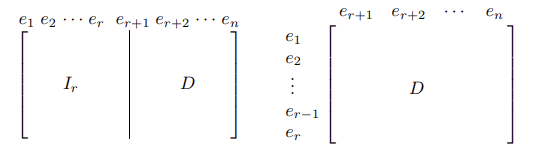
\includegraphics{SRF.png}
    \caption{Standard representative matrices for $M$ (see \cite{oxley1})}
    \label{StandertRepMat}
\end{figure}

Note that in the matrix $[I_r|D]$ from figure (\ref{StandertRepMat}),  only the columns are labelled, but in $D$, both the rows and columns ae labelled.

We can now use this construction to determine the dual of a vector matroid using the following theorem.

\begin{theorem}\label{DualRepMat}
    Let M be the vector matroid of the matrix $[I_r|D]$ where the columns are labelled, in order, $e_1, e_2,\cdots,e_n$ and $1\leq r< n$. Then $M^*$ is the vector matroid of $[-D^T|I_{n-r}]$, where its columns are also labelled $e_1, e_2,\cdots,e_n$ in that order.
\end{theorem}

The following proof was inspired by that in \cite{oxley1}.

\begin{proof}
    We assume that $[I_r|D]$ is as in the contruction of the theorem above. Then $[-D^T|I_{n-r}]$ is as shown in figure (\ref{MatRepresentationDual}).
    \begin{figure}[h]
        \centering
        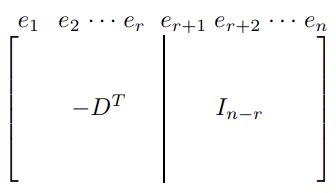
\includegraphics{VMRDual.png}
        \caption{Standart representative form of the dual of a matroid as established in theorem (\ref{DualRepMat}) (see \cite{oxley1}).}
        \label{MatRepresentationDual}
    \end{figure}

    Let $B$ be a basis of $M$. We need to show that $E-B$ is a basis of the vector matroid of $[-D^T|I_{n-r}]$. We can rearrange the columns of $[-D^T|I_{n-r}]$, such that $B=\{e_1,\dots,e_s, e_{r+1}, \dots, e_{r+(r-s)}$\}, for some $s \leq r$. This is possible because we know that it does not affect the corresponding matroid, so the only change it bring to rearrange rows and columns of $[I_r|D]$ is the rearrange of columns and rows of $[-D^T|I_{n-r}]$. 
    
    Using this, we can partition $[I_r|D]$ and $[-D^T|I_{n-r}]$ in the following form
    \begin{align*}
    \begin{bmatrix}
    I_s & 0 & D_{11} & D_{12}\\
    0 & I_{r-s} & D_{21} & D_{22}\\
    \end{bmatrix}
    % 
         \rightarrow 
    \begin{bmatrix}
    -D_{11}^T & -D_{21}^T & I_{r-s} & 0\\
    -D_{12}^T & -D_{22}^T & 0 & I_{n-(2r-s)}\\
    \end{bmatrix}
    \end{align*}
    We will analyze the way $[I_r|D]$ is partitioned. Here, we make the partitioning such that the first component $I_s$ has columns $(e_1 \dots e_s)$, $I_{r-s}$ has columns $(e_{s+1} \dots e_r)$, $D_11$ and $D_21$ have columns $(e_{r+1} \dots e_{2r-s})$, and finally, $D_{12}$ and $D_{22}$ have columns $(e_{(2r-s)+1} \dots e_n)$.
    
    We have that $B$ is a base. This means that it must have the same size as $I_r$. Due to the way the matrix $[I_r|D]$ is partitioned, if we take the components in the partition that contain the column components in the basis, we get the following matrix
        \begin{align*}
        \begin{bmatrix}
        I_s & D_{11}\\
        0 & D_{21}\\
        \end{bmatrix}
        \end{align*}

    As this matrix has the partition components that contain all the elements in the basis, it must have a $rank$ of $r$ (the $rank$ of $[I_r|D]$). Here $r(I_s) = s$, as it is the identity matrix, hence $r(D_{21})=r-s$, which also corresponds to the rank of $-D_21^T$.
    
    If we now observe the partition of $[-D^T|I_{n-r}]$, this will give the same partition lengths in each component as the ones mentioned for $[I_r|D]$ above. That is, the first component $-D_{11}^T$ and $-D_{12}^T$ have columns $(e_1 \dots e_s)$. The components $-D_{22}^T$ and $-D_{21}^T$ have columns $(e_{s+1} \dots e_r)$, $I_{r-s}$ has columns $(e_{r+1} \dots e_{2r-s})$, and finally $ I_{n-(2r-s)}$ has columns $(e_{(2r-s)+1} \dots e_n)$.

    As this time we are dealing with the dual, instead of taking the components that contain the elements in the basis like before, we take the components in the partition of $[-D^T|I_{n-r}]$ that contain the complement of the elements in the basis. Therefore, we obtain the matrix
    \begin{align*}
        \begin{bmatrix}
        -D_{21}^T & 0\\
        -D_{22}^T & I_{n-(2r-s)}\\
        \end{bmatrix}
    \end{align*}

   The rank of this submatrix is the sum of the ranks of $I_{n-(2r-s)}$ and $-D_{21}^T$. We have previously stated that the rank of $-D_{21}^T$ is the same as the one of $D_{21}$. That is, $r(-D_{21}^T)= r-s$, and the $rank$ of $I_{n-(2r-s)}$ is $n-(2r-s)$, which means the total rank is 
   \begin{align*}
    (r-s)+(n-(2r-s))= r-s+n-2r+s = n-r.
   \end{align*}

    This implies that $E-B$ is a basis of the vector matroid of $[-D^T|I_{n-r}]$, since $|E|= n$ and $|B|= r$. This corresponds to the definition of the dual, whose basis $B^*$ must satisfy $|B^*|= n-r$, which holds in this case. This argument could be easily extended to show that every basis of the matroid appears in this way. Therefore, $[-D^T|I_{n-r}]$ is indeed a representation of $M^*$.
\end{proof}

By convention, the form $[-D^T |I_{n-r}]$ is used instead of $[D^T |I_{n-r}]$. However, it is important to remark that this does not bring any issues, because the use of \textit{elementary row operations} does not affect the matroid of a matrix. 

A remarkable result follows almost directly from theorem (\ref{DualRepMat}):

\begin{corollary} \label{corollaryrepdual}
    If a matroid $M$ is \textit{representable} over a field $\mathbb{F}$, then $M ^* $ is also representable over the same field $\mathbb{F}$.
\end{corollary}

\begin{proof}
    Let us prove the Corollary above. Suppose we have a matroid $M$ with rank $m$. That is, the bases of $M$ have size $m$. Then, by assumption, we can say (without loss of generality) that $M$ can be represented by some $m \times n$ matrix $H$ (with $1\leq n < m$), such that $H=[I_{m}|D_{m \times (n-m)}]$ over $\mathbb{F}$. By theorem (\ref{DualRepMat}), its dual is then represented by 
    \begin{align*}
    H^*=[-D^T|I_{(n-m) \times (n-m)}]=[-D_{(n-m) \times m}|I_{(n-m)}],
    \end{align*}
    which is also a matrix over $\mathbb{F}$.
\end{proof}

\begin{exmp}
    Consider the vector matroid $M$ with the following representation over $rrea $
    \begin{align*}
        A = \begin{bmatrix}
            1 & 0 & 0 & 1 & 0 & 1 \\
            0 & 1 & 0 & 1 & -1 & 0 \\
            0 & 0 & 1 & 0 & 1 & 1 \\
        \end{bmatrix}
    \end{align*}

Then, by theorem (\ref{DualRepMat}), the corresponding dual matroid $M^*$ is the vector matroid represented by 
\begin{align*}
        A^* = \begin{bmatrix}
            -1 & -1 & 0 & 1 & 0 & 0 \\
            0 & 1 & -1 & 0 & 1 & 0 \\
            -1 & 0 & -1 & 0 & 0 & 1 \\
        \end{bmatrix}
\end{align*}

As an interesting note, the vector matroid $M$ with matrix representation $A$ is associated to the graph $K_4$. In other words, this means that the matrix $A$ and the graph $K_4$ (figure (\ref{K4Graph})) produce the same matroid.

       \begin{figure}[H]
        \centering
            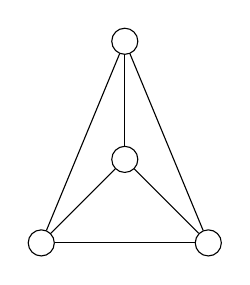
\begin{tikzpicture}[
                node distance = 15mm and 15mm,
                V/.style = {circle, draw, fill=white!30},
                every edge quotes/.style = {auto, font=\footnotesize, sloped}
                    ]
                \begin{scope}[nodes=V]
                \node (1) {}; 
                \node (2) [below of=1] {}; 
                \node (3) [below left of=2] {}; 
                \node (4) [below right of=2] {}; 
                \end{scope}
                \draw (1) to (2); 
                \draw (1) to (3);
                \draw (1) to (4); 
                \draw (2) to (3);
                \draw (2) to (4); 
                \draw (3) to (4);
            \end{tikzpicture}
            \caption{$K_4$, the complete graph on 4 vertices.}
            \label{K4Graph}
        \end{figure}

    Additionally, we can also verify the \textit{rank} and \textit{corank} propositions established before (theorem (\ref{RankAndCorankEquation})). That is, we can clearly observe that $A$ has a ground set $E=\{e_1, e_2, \dots, e_6\}$ with $6$ elements, where each $e_i; i =1,2, \cdots,6$ represents a column, hence $|E|=6$. We also see that $A$ has rank $r(A)=3$, which can be easily verified by observing the first $3$ columns that correspond to the identity matrix in the construction of the form $[I_r|D]$. Similarly, if we observe the dual, we notice that $r(A^*)=3$ as well. We conclude that 
    \begin{align*}
    r(A)+r(A^*)= 3 + 3 = 6 = |E|
    \end{align*}
\end{exmp}

%

\subsection{Dual of graphic matroids}
We have studied many concepts related to dual matroids, including some representations for vector matroids. We have however not gone into detail with regard to graphic matroids. We then pose the question --- \textit{``Is it possible to have a graphic matroid whose dual is not graphic?"}

To answer this question, we formulate the following theorem

\begin{theorem}
    The dual of a graphic matroid is itself graphic if and only if the underlying graph is planar.
\end{theorem}

The proof for this theorem is outside the scope of this article. A proof can be found in \cite[section 2.4]{oxley1}.

\begin{exmp}
    Let us consider the bipartite graph $K_{3,3}$.
\begin{figure}[H]
\centering
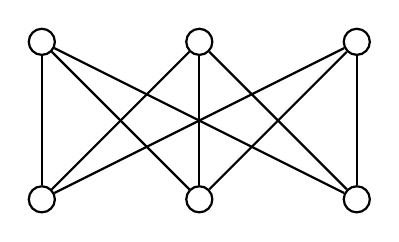
\begin{tikzpicture}[node distance={20mm}, thick, main/.style = {draw, circle}] 
    \node[main] (1) {}; 
    \node[main] (2) [below of=1] {}; 
    \node[main] (3) [right of=1] {}; 
    \node[main] (4) [below of=3] {}; 
    \node[main] (5) [right of=3] {}; 
    \node[main] (6) [below of=5] {}; 
    \draw (1) to (2); 
    \draw (1) to (4);
    \draw (1) to (6); 
    \draw (3) to (2);
    \draw (3) to (4); 
    \draw (3) to (6);
    \draw (5) to (2); 
    \draw (5) to (4);
    \draw (5) to (6);
    \end{tikzpicture}
    \caption{The bipartite graph $K_{3,3}$}
    \label{fig:enter-label}
\end{figure}

This graph has $9$ edges, which means it has $E=\{1,2,3, \dots, 9\} $ as its ground set. The matrix associated to the matroid $M(K_{3,3})$ is the following:
\begin{align*}
J = \begin{bmatrix}
    1 & 0 & 0 & 0 & 0 & 1 & 0 & 0 & 1\\
    0 & 1 & 0 & 0 & 0 & 1 & 1 & 0 & 1\\
    0 & 0 & 1 & 0 & 0 & 1 & 1 & 1 & 1\\
    0 & 0 & 0 & 1 & 0 & 0 & 1 & 1 & 1\\
    0 & 0 & 0 & 0 & 1 & 0 & 0 & 1 & 1\\
\end{bmatrix}
\end{align*}

    This is the case because labelling the columns of $J$ as $E = \{e_1,\dots, e_9\}$ and defining a matroid $M(J)$ on $E$, lets us associate each column of $J$ to the correspondingly labeled edge in $K_{3,3}$ so they generate the same matroid. Moreover, this means that we can take a basis for the column space of $J$, such as $B = \{e_1, e_2, e_3, e_4, e_5\}$, that corresponds to a spanning tree $T$ of $K_{3,3}$ (see figure (\ref{K33STE})). In other words, this means that adding any other column to $J$ yields a linear dependency (more precisely, a circuit in $M(J)$), and adding any edge to $T$ generates a cycle.

\begin{figure}[H]
    \centering
    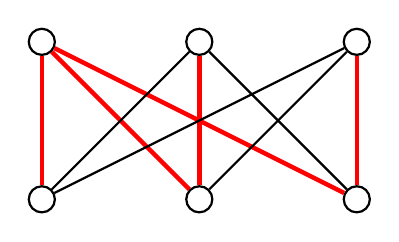
\begin{tikzpicture}[node distance={20mm}, thick, main/.style = {draw, circle}] 
        \node[main] (1) {}; 
        \node[main] (2) [below of=1] {}; 
        \node[main] (3) [right of=1] {}; 
        \node[main] (4) [below of=3] {}; 
        \node[main] (5) [right of=3] {}; 
        \node[main] (6) [below of=5] {}; 
        \draw [ultra thick,red] (1) to (2); 
        \draw [ultra thick,red] (1) to (4);
        \draw [ultra thick,red] (1) to (6); 
        \draw (3) to (2);
        \draw [ultra thick,red] (3) to (4); 
        \draw (3) to (6);
        \draw (5) to (2); 
        \draw (5) to (4);
        \draw [ultra thick,red] (5) to (6);
    \end{tikzpicture}
    \caption{Graph $K_{3,3}$, showing in red an example of edges that form a spanning tree, that can be associated accordingly to the basis of $J$.}
    \label{K33STE}
\end{figure}

Now that we have show that $K_{3,3}$ has an associated matrix, which produces the same matroid, we can use theorem (\ref{DualRepMat}) to obtain the corresponding dual:
\begin{align*}
  J^*=\begin{bmatrix} 
1 & 1 & 1 & 0 & 0 & 1 & 0 & 0 & 0\\
0 & 1 & 1 & 1 & 0 & 0 & 1 & 0 & 0\\
0 & 0 & 1 & 1 & 1 & 0 & 0 & 1 & 0\\
1 & 1 & 1 & 1 & 1 & 0 & 0 & 0 & 1\\
\end{bmatrix}
\end{align*}

As a sanity check, we can see that $r(J) = 5$,  $r^*(J)=4$, and $|E(M)|=9$. We then notice the following does indeed hold:
\begin{align*}
r(M) + r^*(M) = |E(M)|.
\end{align*}

According to corollary (\ref{corollaryrepdual}), \textit{If a matroid \textit{M} is \textit{representable} over a field $\mathbb{F}$, then \textit{M*} is also representable over $\mathbb{F}$}. Here we see that both matroids are vector matroids over the field $\mathbb{F}_2$. 

Finally, we can observe that $K_{3,3}$ is not a planar graph. This implies that, although $M(K_{3,3})$ is a graphic matroid, its dual ($M^*(K_{3,3})$) is not graphic.
\end{exmp}
